%% Lines to compile only this capter
% \documentclass[11pt, twoside, a4paper, openright]{report}
% \usepackage[utf8]{inputenc}
% \DeclareUnicodeCharacter{223C}{~}

%Bibliography style
% \usepackage[square, numbers]{natbib}
% \usepackage[round]{natbib}
% \usepackage{biblatex}
% \bibliographystyle{unsrtnat}
% \bibliographystyle{unsrt}
% \bibliographystyle{plain}
% \bibliographystyle{aa}
% \usepackage[backend=bibtex,style=authoryear,natbib=true]{biblatex} 
\usepackage[
backend=biber,
style=authoryear,
citestyle=authoryear,
url=false
]{biblatex}
\addbibresource{../source/library.bib}

\usepackage[T1]{fontenc}
\usepackage[french]{babel}
\usepackage{csquotes}  % used for citations (recommended when using biblatex)
%\usepackage{helvet}
%\renewcommand{\familydefault}{\sfdefault}
\usepackage{mathptmx}
\usepackage{amssymb}
\usepackage{geometry} 
\usepackage{xcolor}
\usepackage[absolute,overlay]{textpos}
\usepackage{graphicx}
\usepackage{lipsum}
\usepackage[explicit]{titlesec}
\usepackage{lmodern}
\usepackage{color}
\usepackage{array}
\usepackage{mathtools}
\usepackage{caption}
\usepackage{multicol}
\usepackage{booktabs}
\usepackage{enumitem}
\usepackage{hyperref}
\usepackage{afterpage}
\usepackage{emptypage}
\usepackage{setspace}
\usepackage{pgffor}
    \setlength{\columnseprule}{0pt}
    \setlength\columnsep{10pt}
\usepackage[francais,nohints]{minitoc}
    \setcounter{minitocdepth}{3}
 
 %https://la-bibliotex.fr/2019/02/03/ecrire-les-nombres-et-les-unites-avec-latex/   
\usepackage{siunitx}
% \sisetup{
%     detect-all,
%      output-decimal-marker={,},
%      group-minimum-digits = 3,
%      group-separator={~},
%      number-unit-separator={~},
%      inter-unit-product={~},
%      list-separator = {, },
%      list-final-separator = { et },
%      range-phrase = --,
%      separate-uncertainty = true,
%      multi-part-units = single,
%      list-units = single,
%      range-units = single
%     }
\usepackage{physics}
\usepackage{isotope}

\usepackage[perpage]{footmisc} % to reset the counter of footnote each page

    
\usepackage{fancyhdr}			% Entête et pieds de page. Doit être placé APRES geometry
\pagestyle{fancy}		% Indique que le style de la page sera justement fancy
%\lfoot[\thepage]{} 		% gauche du pied de page
%\cfoot{} 			% milieu du pied de page
%\rfoot[]{\thepage} 
\fancyfoot{} % vide le pied~de~page
\fancyfoot[LE,RO]{\thepage}
\fancyfoot[LO,CE]{}% droite du pied de page
\fancyhead{}	
\fancyhead[LE]{\leftmark}	
\fancyhead[RO]{\rightmark}

\fancypagestyle{plain}{%
\fancyhf{} % vide l’en-tête et le pied~de~page.
\fancyfoot[LE,RO]{\thepage} % numéro de la page en cours en gras% et centré en pied~de~page.
\renewcommand{\headrulewidth}{0pt}
\renewcommand{\footrulewidth}{0pt}}



% Premiere page des chapitres
\newlength\chapnumb
\setlength\chapnumb{3cm}
 
\titleformat{\chapter}[block] {
  \normalfont}{}{0pt} { %police
    \parbox[b]{\chapnumb}{
      \fontsize{120}{110}\selectfont\thechapter} %taille du chiffre
      \parbox[b]{\dimexpr\textwidth-\chapnumb\relax}{
        \raggedleft 
        \hfill{\bfseries\Huge#1}\\ %taille du titre
        \rule{\dimexpr\textwidth-\chapnumb\relax}{0.4pt} %ligne de separation
  }
}
 
 %premiere page chapitre non numerote (remerciement, table des matieres ...)
 
\titleformat{name=\chapter,numberless}[block]
{\normalfont}{}{0pt}
{   
    \parbox[b]{\dimexpr\textwidth}{%   
    \hfill{\bfseries\Huge#1}\\
  \rule{\dimexpr\textwidth}{0.4pt}}}
    
 %   \titleformat{name=\chapter,numberless}[block]
%{\normalfont}{}{0pt}
%{\parbox[b]{\chapnumb}{%
%   \mbox{}}%
%  \parbox[b]{\dimexpr\textwidth-\chapnumb\relax}{%
%    \raggedleft%
%    \hfill{\bfseries\Huge#1}\\
%    \rule{\dimexpr\textwidth-\chapnumb\relax}{0.4pt}}}


%%%    SIunitx
\sisetup{locale = FR,
  % inter-unit-product=\ensuremath{\cdot},
  inter-unit-product=\ensuremath{\,},
  per-mode=reciprocal,
  separate-uncertainty = true,
  detect-all
}
\DeclareSIUnit{\Mpc}{Mpc}
\DeclareSIUnit{\kpc}{kpc}
\DeclareSIUnit{\Gpc}{Gpc}
\DeclareSIUnit{\h}{\textit{h}~}
\DeclareSIUnit{\perh}{\textit{h}^{-1}\,}

%%% Geometry
\geometry{
left=20mm,
top=30mm,
right=20mm,
bottom=30mm
}

%%% Color
\definecolor{bordeau}{rgb}{0.3515625,0,0.234375}

%%% Commands
\newcommand{\Nmocks}{\num{30}}
\newcommand{\hMpc}{h^{-1}\,\mathrm{Mpc}}
\newcommand{\hGpc}{h^{-1}\,\mathrm{Gpc}}
\newcommand{\kms}{\mathrm{km\,s^{-1}}}

\newcommand{\lya}{Ly$\alpha$}
\newcommand{\lyb}{Ly$\beta$}
\newcommand{\lyalya}{Ly$\alpha$(Ly$\alpha$)}
\newcommand{\lyalyb}{Ly$\alpha$(Ly$\beta$)}

\newcommand{\lrf}{\lambda_{\rm RF}}
\newcommand{\kpar}{k_{\parallel}}
\newcommand{\apar}{\alpha_{\parallel}}
\newcommand{\rpar}{r_{\parallel}}
\newcommand{\aperp}{\alpha_{\perp}}
\newcommand{\rperp}{r_{\perp}}
\newcommand{\kperp}{k_{\perp}}

\newcommand{\blya}{b_{\rm Ly\alpha}}
\newcommand{\betalya}{\beta_{\rm Ly\alpha}}
\newcommand{\blyb}{b_{\rm Ly\alpha}}
\newcommand{\betalyb}{\beta_{\rm Ly\beta}}
\newcommand{\dlya}{d_{\rm Ly\alpha}}
\newcommand{\bhcd}{b_{\rm HCD}}
\newcommand{\betahcd}{\beta_{\rm HCD}}
\newcommand{\Fhcd}{F_{\rm HCD}}
\newcommand{\Lhcd}{L_{\rm HCD}}

\newcommand{\imin}{i_{\rm min}}
\newcommand{\imax}{i_{\rm max}}
\newcommand{\jmin}{j_{\rm min}}
\newcommand{\jmax}{j_{\rm max}}

\newcommand{\xioned}{\xi_{\rm 1d}}
\newcommand{\DHub}{D_{H}}
\newcommand{\DM}{D_{M}}

\newcommand{\omegam}{\Omega_M}
\newcommand{\omegac}{\Omega_C}
\newcommand{\omegab}{\Omega_B}
\newcommand{\omegan}{\Omega_\nu}
\newcommand{\omegal}{\Omega_\Lambda}
\newcommand{\omegak}{\Omega_k}
\newcommand{\orad}{\Omega_R}
\newcommand{\ogam}{\Omega_\gamma}
\newcommand{\lcdm}{$\Lambda$CDM}

\newcommand{\picca}{\texttt{picca}}

%%% Rem's command
\newcommand\blankpage{%
    \null
    \thispagestyle{empty}%
    \addtocounter{page}{-1}%
    \newpage}
  
% Command to set up a particular alignment for a cell in tabular :
% \myalign{c}{foo} for instance
\newcommand*{\myalign}[2]{\multicolumn{1}{#1}{#2}}
 
\renewcommand{\thesection}{\arabic{section}}

% Romain
\newcommand{\cRM}[1]{\MakeUppercase{\romannumeral #1}}	% Capital
\newcommand{\cRm}[1]{\textsc{\romannumeral #1}}	% Petit majuscule
\newcommand{\crm}[1]{\romannumeral #1}
% Siècle %
\newcommand{\siecle}[1]{\cRm{#1}\textsuperscript{e}~siècle}



% Thesis title
\newcommand{\PhDTitle}{Les forêts \lya{} du relevé eBOSS : comprendre les fonctions de corrélation et les systématiques} 

% Name
\newcommand{\PhDname}{Thomas Etourneau} 

% Change this variable if you add or remove chapters
\newcommand*{\NumOfChapters}{6}

% Change this variable if you add or remove appendices
\newcommand*{\NumOfAppendices}{2}

% PDF metadata
\hypersetup{
	pdfauthor={\PhDname},
	pdfsubject={Manuscrit de thèse de doctorat},
	pdftitle={\PhDTitle}
}


% \begin{document}
%%

\chapter{Le relevé eBOSS de SDSS}
\minitoc
\newpage
\thispagestyle{fancy}
\graphicspath{ {../figures/eBOSS/} }

\section{Le Sloan Digital Sky Survey}


Le \emph{Sloan Digital Sky Survey} (SDSS) est né dans les années 1990 de l'ambition de réaliser un relevé spectroscopique à la fois profond et étendu dans le but d'étudier, entre autres, la structuration de l'univers à grande échelle. Cette idée a été rendue possible par l'apparition des capteurs CCD, des spectrographes à fibres optiques ainsi que par les capacités à analyser des lots de données de plus en plus grands. En 1991, la fondation Sloan décide donc d'investir dans ce projet ambitieux, permettant sa construction et lui donnant ainsi son nom. 
Le téléscope fut construit à l'Apache Point Observatory (APO) au Nouveau Mexique, et la première lumière prise en 1998. Ce télescope capable de mesurer le spectre de centaines d'objets à la fois, générant ainsi de grandes quantités de données, a marqu\'e une nouvelle ère, à la fois en terme de relevé cosmologique et de manière d'analyser de telles quantités de donnés.

\subsection{SDSS I-II-III}
Les deux premières générations du SDSS, SDDS-I de 2000 à 2005 puis SDSS-II de 2005 à 2008, ont produit plusieurs résultats importants.\\
Premièrement, un relevé photométrique multi-bandes de plus de $\SI{11600}{\square\deg}$, couvert par les filtres \emph{u, g, r, i} and \emph{z}\footnote{Ces filtres couvrent les longueurs d'onde allant de $400$ à $1000\,\mathrm{nm}$. Voir~\ref{fig:Filtres}}. Parmis ces $\SI{11600}{\square\deg}$, \num{7500} forment le relevé contigu appelé \emph{the Legacy Survey}. Ce relevé photométrique a permis de sélectionner plus de \num{930000} galaxies et \num{120000} quasars candidats, afin d'en mesurer les spectres. Il a été rendu public lors de la septième plublication de données de SDSS\footnote{SDSS DR7 : http://www.sdss.org/dr7} et est détaillé dans \textcite{Abazajian2008}. Son étude a conduit à la première détection à $3,6\,\sigma$ des BAO \autocite{Eisenstein2005}, mesurant ainsi l'échelle BAO moyennée sur le volume, $D_V$, à un redshift effectif de \num{0,35} et avec une précision de \SI{5}{\percent}. \\
Un second relevé photométrique et spectroscopique de $\SI{3500}{\square\deg}$, contenant \num{460000} étoiles de notre galaxie, a été produit dans le but d'étudier la structure et la composition de la Voie Lactée. Ce relevé est nommé \emph{SEGUE} (Sloan Extension for Galactic Understanding and Exploration \autocite{Collaboration2009}.\\
Enfin, le \emph{SDSS Supernova Survey}, un relevé d'environ $\SI{250}{\square\deg}$ observé à plusieurs reprises et visant à contraindre l'accélération de l'expansion de l'univers grâce à l'étude des supernovae de type 1a, a produit un échantillon d'environ 500 SNe 1a, toutes confirmées spectroscopiquement entre $z=\num{0,1}$ et $z=\num{0,4}$.

\paragraph{}
Au vu du succès de SDSS-I et II, une troisième géneration de SDSS débuta fin 2008. Elle se compose de 4 relevés différents \autocite{Eisenstein2011}, avec le même téléscope que les deux générations précédentes. \\
Parmi ces relevés figure \emph{SEGUE-2}, suite du programme SEGUE. Il a produit un relevé d'étoiles de la Voie Lactée dans le but de mieux comprendre la formation et l'évolution de notre galaxie. Le relevé \emph{MARVEL} (Multi Object APO Radial Velocity Exoplanet Large-ara Survey) a opéré de 2008 à 2012. Ce programme étudie les exo-planètes via deux spectrographes interférométrique de 60 fibres chacun, en mesurant la vitesse radiale d'environ \num{11000} étoiles brillantes. \emph{APOGEE-1}, pour APO Galactic Evolution Experiment 1, vise à mieux comprendre la formation et l'évolution de notre galaxie. Il a produit un relevé spectrométrique dans l'infra rouge de très haute résolution et très haut rapport signal sur bruit d'environ \num{150000} étoiles. Ce relevé ainsi que celui de SEGUE-2 jouent un rôle important dans la compréhension de la formation de notre galaxie et dans l'étude de la distribution de matière noire à petite échelle.\\
Enfin, le 4e relevé de SDSS-III est nommé \emph{BOSS}, pour Baryon Oscillation Spectroscopic Survey. Il poursuit la mesure de l'échelle BAO faite avec le Legacy Survey et inclut un nouveau traceur : la forêt Lyman alpha dans le spectre de quasars lointains. Afin d'observer un plus grand nombre d'objets et d'avoir une mesure plus précise, le spectrographe initialement présent sur SDSS a été amélioré : la gamme de longueur d'onde observée est plus grande, le diamètre des fibres a été réduit, ce qui conduit à un nombre total de \num{1000} fibres. Les observations commencèrent en 2009 et se terminèrent, en avance, en 2014. Le temps d'observation restant permit de mener plusieurs programmes d'observation en dark time\footnote{Le dark time correspond au moment ou le ciel est le plus sombre et le plus propice à observer des objets peu lumineux.}, tel que \emph{SEQUELS} (Sloan Extended QUasars, ELG and LRG Survey) qui a réalisé un relevé de $\SI{300}{\square\deg}$ avec le spectrographe de BOSS, afin de tester la sélection des cibles pour SDSS-IV.\\
BOSS mena à de nombreux résultats importants.
Il produisit un relevé de plus de 1,5 million de galaxies, qui donna une mesure de $D_{\mathrm{M}}$ avec une précision de \SI{2.0}{\percent} et une mesure de $D_{\mathrm{H}}$ avec une précision de \SI{3.2}{\percent} à un redshift $z=\num{0,38}$, une mesure de $D_{\mathrm{M}}$ avec une précision de \SI{1.9}{\percent} et une mesure de $D_{\mathrm{H}}$ avec une précision de \SI{3.0}{\percent} à $z=\num{0,51}$, ainsi qu'une mesure de $D_{\mathrm{M}}$ avec une précision de \SI{1.9}{\percent} et une mesure de $D_{\mathrm{H}}$ avec une précision de \SI{3.0}{\percent} à $z=\num{0,61}$ \autocite{Alam2016}.
L'étude du \lya{} conduisit à une mesure de $D_{\mathrm{M}}$ avec une précision de \SI{4}{\percent} et une mesure de $D_{\mathrm{H}}$ avec une précision de \SI{4.8}{\percent} à un redshift effectif $z=\num{2,4}$ \autocite{Bourboux2019}.
L'ensemble des données de SDSS-III a été rendu public lors de la douzième publication de données de SDSS\footnote{SDSS DR12 : http://www.sdss.org/dr12} \autocite{Alam2015}.


\subsection{SDSS-IV}

La quatrième génération de SDSS débuta courant 2014. Elle comporte 3 programmes spectroscopiques majeurs \autocite{Blanton2017}, dont nous donnons une brève description ici :
\begin{itemize}
\item \emph{APOGEE-2}, suite d'APOGEE-1, effectue de la spectroscopie stellaire grâce à un spectrographe de haute résolution dans le proche infrarouge. En plus du relevé dans le \emph{NGC} (North Galactic Cap) mené à l'APO, le programme comporte un relevé dans le \emph{SGC} (South Galactic Cap). Le relevé sud est produit grâce au télescope du Pont, de \num{2,5} mètres, situé à Las Campanas au Chili. L'objectif final est d'obtenir le spectre de plus de \num{400000} étoiles dans le proche infrarouge, afin d'accéder aux régions clés de la Voie Lactée non-observable en optique, et ainsi mieux comprendre la formation et l'évolution des galaxies.
\item \emph{MaNGA} est un nouveau programme de SDSS. C'est le premier à utiliser un spectrographe de champ intégré\footnote{\emph{intregral field spectrograph} en anglais}. Contrairement aux programmes précédents qui obtenaient le spectre du centre de la galaxie cible, MaNGA va mesurer le spectre en plusieurs points répartis sur toute la surface de la galaxie observée. Ce procédé va permettre d'étudier la structure interne d'environ \num{10000} galaxies proches ($z < \num{0,03}$), en mesurant notamment les cartes des vitesses dans le plan transverse à la ligne de visée et des dispersions de vitesse des étoiles, ainsi que leur  métallicité.
\item \emph{eBOSS} pour Extended Baryon Oscillation Spectroscopic Survey, est le troisième programme majeur de SDSS-IV. C'est le programme qui fournit les données de ce manuscrit, il est décrit en détail dans la section suivante ainsi que dans \textcite{Dawson2015}. En plus du programme principal, eBOSS inclut deux sous-programmes : \emph{SPIDERS} et \emph{TDSS}.
  
  SPIDERS étudie la nature des émissions en X. Il utilise \SI{5}{\percent} des fibres d'eBOSS afin de viser des sources émettant en X. Ces sources sont issues principalement du relevé \emph{ROSAT All Sky Survey} ainsi que des sources observées par le satellite \emph{eROSITA}.

  TDSS vise à comprendre la nature des sources variables. Il utilise lui aussi \SI{5}{\percent} des fibres d'eBOSS, afin de mesurer le spectre de sources variables présentes dans le relevé \emph{Pan-STARRS1} (PS1) ou dans l'imagerie de SDSS. Parmi les sources identifiées par PS1, environ \SI{60}{\percent} sont des quasars, et \SI{40}{\percent} des étoiles variables. A la fin, TDSS aura produit un relevé d'environ \num{200000} spectres, jusqu'à une magnitude\footnote{La magnitude est une mesure de la luminosité des objets célestes. Elle est construite sur une échelle logarithmique inversée : plus la magnitude est importante, et moins l'objet est lumineux.} limite de 21.
\end{itemize}



\section{eBOSS}

Suite au succès de BOSS, la collaboration SDSS poursuit la mesure de l'échelle BAO avec le programme eBOSS. Celui-ci inclut deux nouveaux traceurs, afin de sonder une époque clé qui est l'époque de transition de la domination de la matière à celle de l'énergie noire.
L'objectif principal est d'étendre la mesure de distance effectuée avec les galaxies de BOSS à un redshift $\num{0,6} < z < \num{1}$, ainsi que de permettre la première analyse RSD\footnote{Les analyses RSD désignent les analyses qui visent à mesurer le taux de croissance $f$ afin de contraire la gravité.} à l'aide de quasars en tant que traceurs et la première mesure de l'échelle BAO à un redshift $1 < z < 2$.
La précision visée sur la mesure de distance avec l'échantillon de galaxies est de \SI{1}{\percent}, et de \SI{2}{\percent} pour les nouveaux traceurs.



\subsection{Les traceurs de eBOSS}

Afin d'étendre la gamme de redshift sondée par BOSS, eBOSS inclut donc deux nouveaux traceurs : les ELG et les quasars en tant que traceurs de la matière. Auxquels s'ajoutent les traceurs déja présents dans BOSS : les LRG et les forêts \lya{} des quasars. Ces traceurs sont présentés ici :
\begin{itemize}
\item LRG : l'échantillon de \emph{Luminous Red Galaxies} déja observé lors du programme BOSS est étendu. Un minimum de \num{300000} galaxies dont le redshift est mesuré spectroscopiquement sont nécessaires dans la gamme de redshift $\num{0,6} < z < \num{1}$ afin d'atteindre la précision de \SI{1}{\percent} sur l'échelle BAO.
\item ELG (\emph{Emission Line Galaxies}) : ce sont des galaxies bleues formant beaucoup d'étoiles, facilement identifiables par leurs raies d'émission. Leur relevé couvre les redshifts $\num{0,6} < z < \num{1,1}$ et doit conduire à une mesure à \SI{2}{\percent} de précision de l'échelle BAO.
\item QSO : nouveaux traceurs, ils sont utilisés afin de construire un relevé spectroscopique au même titre que les LRG, mais à plus grand redshift. Ils permettent ainsi de mener une analyse RSD et de mesurer l'échelle BAO dans une époque jusque là insondée ($\num{0,9} < z < \num{2,2}$). Cet échantillon peu dense doit mener à une mesure à \SI{2}{\percent} sur l'échelle BAO. Du fait que ce relevé est dominé par le bruit de grenaille (\emph{shot noise}), de futurs relevés pourront venir le compléter et ainsi augmenter la précision statistique de la mesure.
\item \lya{} QSO : ces quasars sont les objets dont les spectres fournissent la forêt \lya{}. Contrairement aux traceurs directs, la quantité d'information contenue dans la forêt \lya{} dépend du rapport signal sur bruit. Les quasars \lya{} de BOSS possédant un faible rapport signal sur bruit sont donc réobservés dans eBOSS. Le gain attendu sur le rapport signal sur bruit grâce à cette réobservation est d'environ \SI{40}{\percent}. La densité moyenne de ces objets est de l'ordre de $\SI{8}{deg^{-2}}$. \\
  En plus de ces objets, eBOSS a observé de nouveaux quasars \lya{}, avec une densité moyenne de $\SI{6}{deg^{-2}}$.
\end{itemize}
La répartition en redshift de ces quatre traceurs est représentése sur la figure~\ref{fig:eBOSStracers}.
\begin{figure}
  \centering
  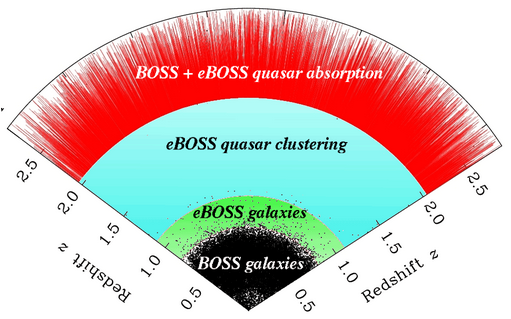
\includegraphics[scale=0.5]{eBOSStracers}
  \caption{Représentation des quatre différents traceurs d'eBOSS et leur r\'epartition en redshift.}
  \label{fig:eBOSStracers}
\end{figure}
\paragraph{}
Le relevé produit par eBOSS contient un échantillon de LRG couvrant la gamme $\num{0,6} < z < \num{1}$ avec une densité de 60 cibles par $\si{\square\deg}$ dont la pureté est supérieure à \SI{80}{\percent}. L'échantillon d'ELG couvre une gamme en redshift légèrement plus haute et contient un total de \num{173736} objets ($\sim\,\SI{130}{deg^{-2}}$). Les quasars utilisés dans les analyses RSD constituent un échantillon couvrant la gamme $\num{0,9} < z < \num{2,2}$ avec une densité de 90 cibles par $\si{\square\deg}$ dont la pureté est supérieure à \SI{50}{\percent}. Enfin, eBOSS fournit \num{60000} nouveaux quasars \lya{} ainsi que la réobservation de \num{60000} quasars \lya{} déja observés avec BOSS. Pour la suite, nous nous intéresserons uniquement aux quasars \lya{}, qui constituent l'ensemble des données traitées dans cette étude. Ils seront simplement désignés par quasars ou QSO.


% Enfin la réobservation des quasars \lya{} de faible luminosité apportera 8 objets par \si{\square\deg} à des redshifts $z > 2,1$, auxquels s'ajouteront de nouveaux quasars \lya{} avec une densité de 18 objets par \si{\square\deg}. \\
% Pour la suite, nous nous intéresserons uniquement aux quasars \lya{}, qui constituent l'ensemble des données traitées dans cette étude. Ils seront simplement désignés par quasars ou QSO.


\subsection{Sélection des cibles}

La sélection des cibles s'effectue sur la base du relevé photométrique dans les bandes \emph{ugriz} réalisé par SDSS-I et II et rendu publique lors de la neuvième publication de donnée SDSS (DR9\footnote{http://www.sdss.org/dr9}).
Lors de la sélection des cibles de BOSS, la photométrie provenant de \emph{UKIDSS} (UKIRT Infrared Deep Sky Survey, \textcite{Lawrence2006}) et de \emph{GALEX} (Galaxy Evolution Explorer, \textcite{Martin2004}) a été utilisée.
De la même manière, la photométrie de SDSS est complétée par plusieurs relevés afin de définir les nouveaux quasars à observer dans eBOSS :
\begin{itemize}
\item Les bandes W1 et W2 ($\SI{3,4}{\micro\meter}$ et $\SI{4,6}{\micro\meter}$) du relevé photométrique du satellite \emph{WISE} (Wide-field Infrared Survey Explorer, \textcite{Wright2010})
\item La photométrie multi-époque de \emph{PTF} (Palomar Transient Factory, \textcite{Law2009})
\item Les données de \emph{FIRST} (Faint Images of the Radio Sky at Twenty-Centimeters, \textcite{Becker1995})
\end{itemize}

% Contrairement aux relevés d'objets ponctuels tels que les galaxies, les quasars ne nécessitent pas une homogénéïté importante à travers le relevé. Une distribution aléatoire de quasars est suffisante afin de mesurer le champ de densité d'avant plan. Ceci simplifie énormément la sélection des cibles.

% Les relevés d'objets utilisés en tant que traceurs directs pour la mesure de l'échelle BAO ou du \#prov clustering, tels que les relevés de galaxies, nécessitent une très bonne homogénéïté. Contrairement à ces relevés, les quasars utilisés pour le \lya{} ne nécessitent pas cette homogénéïté (\#prov expliquer pourquoi). \\
\paragraph{} Pour BOSS, le relevé de QSO a été construit en utilisant d'une part l'algorithme \texttt{XDQSO} \autocite{Bovy2010a} pour l'échantillon \texttt{QSO\_CORE}, ce qui a permis d'avoir un échantillon homogène, et d'autre part en incluant des QSO sélectionnés via différentes techniques afin d'augmenter au maximum la densité de quasars \lya{}.
Contrairement aux relevés d'objets utilisés en tant que traceurs directs pour la mesure de l'échelle BAO ou les pour les anayses RSD, les quasars \lya{} ne nécessitent pas un relevé homogène (voir l'introduction de la section~\ref{sec:estimateurs}).
C'est pour cette raison que l'échantillon de QSO \lya{} peut être complété sans se soucier de dégrader l'homogénéité.
Cependant, la présence d'un échantillon homogène de quasars à grand redshift permet d'autres sciences que la mesure de l'échelle BAO.
Par exemple, le papier \textcite{Laurent2016} étudie l'homogénéïté cosmique en utilisant l'échantillon de quasars DR12 de BOSS.

% Pour BOSS, le relevé de QSO a été construit en utilisant l'algorithme \texttt{XDQSO} (CITE:Bovy et al. 2011a,b), ce qui a permis d'avoir un relevé homogène. Comme expliqué précédemment, cette homogénéïté n'est pas nécessaire , mais permet d'autres sciences que la mesure de l'échelle BAO avec le \lya{}. Par exemple, le papier~\cite{Laurent2016} étudie l'homogénéïté cosmique en utilisant l'échantillon de quasars DR12 de BOSS.


\paragraph{}
Pour eBOSS, la présence d'un échantillon de quasars à $\num{0,9} < z < \num{2,2}$ destiné à la fois à la mesure de l'échelle BAO et aux analyses RSD permet de relâcher le critère d'homogénéité imposé pour les quasars de BOSS, et ainsi d'augmenter le nombre de cibles de quasars \lya{}.
L'algorithme \texttt{XDQSO} est donc utilisé avec des paramètres moins strictes que pour BOSS, afin d'augmenter la densité de quasars \lya{}.
Ainsi, \num{6,6} nouveaux quasars par $\si{\square\deg}$ sont ajoutés à l'échantillon de cette manière.
Ensuite, les QSO de BOSS ayant un rapport signal sur bruit $\num{0,75} < S/R < \num{3}$ et ne comprenant pas de BAL sont réobservés.
% Ces quasars représentent une densité de cible de $8,3\,\mathrm{deg^{-2}}$.
% A ces quasars s'ajoutent de nouveaux quasars sélectionnés par l'algorithme \texttt{XDQSO}.
% L'algorithme est utilisé avec des paramètres moins strictes que pour BOSS, afin d'augmenter le nombre de cibles.
% $6,6\,\mathrm{deg^{-2}}$ nouveaux quasars sont ainsi ajoutés à l'échantillon.
Enfin, de nouveaux candidats quasars sont sélectionnés gr\^ace aux données de PTF, avec une densité de $\SI{3,2}{deg^{-2}}$. Les catalogues FIRST fournissent eux aussi de nouveaux quasars potentiels, avec une densité de $\SI{1}{deg^{-2}}$.
Ainsi, un total de total d'environ 8 QSO par $\si{\square\deg}$ sera réobservé, accompagné d'environ 18 nouveaux quasars par $\si{\square\deg}$.

% Afin de construire le relevé eBOSS, le même algorithme a été utilisé pour sélectionner les quasars. Cette fois ci, la présence d'un échantillon de quasars à $0.9 < z < 2.2$ destiné à la fois à la mesure de l'échelle BAO et du clustering (\#prov) a permis réduire les critères de sélection des QSO et ainsi de dégrader l'homogénéïté de l'échantillon de quasars \lya{} afin d'augmenter le nombre de cibles. 

% releve de BOSS : destine a la base pour le Lya, donc pas besoin en soit que ca soit homogene, mais ca a ete construit plus ou moins homogene car ca doit simplifier des choses et ca permet de faire d'autre sciences (papier de Pierre Laurent).
% eBOSS : on degrade l'homogeneite pour avoir plus de qso (on s'en fiche puisque c'est pour le lya). et de toute facon on a un releve homogene qu'est le releve QSO CORE 0.9 < z < 2.2 dans eBOSS.

\subsection{Pavage du ciel}

Une fois que les cibles ont été sélectionnées grâce aux observations photométriques, la phase d'observation spectroscopique peut commencer. Les données sont acquises via \num{1000} fibres optiques insérées dans une plaque, que l'on dispose au centre du plan focal du télescope. 
Le processus de ``pavage'' \autocite{Blanton2001} consiste donc à assigner chaque cible ou presque à une fibre optique dans une plaque d'observation, en minimisant le nombre de plaques nécessaires et en maximisant le nombre de cibles qui reçoivent une fibre. Cette opération est réalisée par l'algorithme de sélection des cibles ainsi que du nombre de fibres disponibles. \\
% Le temps d'exposition d'une plaque est de l'ordre de 1,5 heure, ce qui, étant donné le nombre d'heures allouées à eBOSS, permet d'observer environ \num{1800} plaques.
% Chaque plaque couvre une surface de $7{\square\deg}$ sur le ciel. En moyenne, un centre de plaque est assigné tous les $5{\square\deg}$ afin d'éviter les trous dans le relevé. 
% Ainsi, \num{1800} plaques peuvent couvrir un relevé d'environ $\num{9000}{\square\deg}$.
Afin d'observer les $\SI{9000}{\square\deg}$ constituant le relevé d'eBOSS, celui-ci est divisé en environ \num{1800} plaques. Chaque plaque couvre une surface de $\SI{7}{\square\deg}$ sur le ciel, et en moyenne, un centre de plaque est assigné tous les $\SI{5}{\square\deg}$ afin d'éviter les trous dans le relevé. Étant donné le nombre d'heures allouées à eBOSS et le nombre de plaques à observer, chaque plaque est observées durant environ \num{1,5} heure. \\
Parmi les \num{1000} fibres disposées sur chaque plaque, \num{100} sont destinées aux programmes TDSS et SPIDERS et \num{100} fibres supplémentaires sont réservées à la calibration. Il reste donc \num{800} fibres par plaque destinées aux traceurs de eBOSS. Ces fibres sont assignées aux LRG et QSO. Le relevé des ELG se fait sur des plaques indépendantes. Afin de mener ce relevé des ELG, la taille du relevé des LRG et QSO est réduit de \num{9000} à $\SI{7500}{\square\deg}$. Ainsi \num{300} plaques sont rendues disponibles pour l'observation des ELG ($\sim\,\SI{1500}{\square\deg}$).


\paragraph{} Une fois le pavage du ciel effectué, la position des fibres sur le ciel est convertie en coordonnées dans le plan focal du télescope. A cause de la chromaticité de l'instrument, la position dans le plan focal de chaque objet observé dépend de la longueur d'onde. Ainsi chaque fibre dite de science est positionnée de manière à maximiser la lumière en sortie à $\SI{5400}{\angstrom}$ pour les galaxies et les quasars destinés aux analyses RSD, et à $\SI{4000}{\angstrom}$ pour les quasars \lya{}. \\
Parmi les \num{100} fibres allouées à la calibration, \num{80} sont destinées à la soustraction du fond de ciel. Pour chaque plaque, il est requis que chaque spectrographe reçoivent au moins \num{30} fibres de ciel. Les \num{20} fibres restantes sont destinées à la calibration du flux. Celle-ci se fait en pointant des étoiles standards de type F. De la même manière, parmi ces \num{20} fibres, au minimum \num{6} fibres sont requises sur chaque spectrographe.


\subsection{Phase d'observation}

Une fois le pavage du ciel réalisé et la position de chaque fibre dans le plan focale déterminée, les plaques sont préparées puis percées. Ces plaques sont en aluminium de $\SI{3,2}{\milli\meter}$ d'épaisseur et de $\SI{80}{\centi\meter}$ de diamètre. La zone contenant les fibres mesure $65,2\,\mathrm{cm}$ de diamètre. La préparation des plaques est faite à l'université de Washington. Elle est décrite dans \textcite{Blanton2017}.\\
Une fois les plaques prêtes, les observations peuvent commencer. La prise de données a débuté en juillet 2014. Pendant les deux premières années, seules les plaques des LRG et des QSO ont été observées. Les deux années suivantes, les plaques des ELG ont été observées en alternance avec les plaques assignées aux LRG et QSO. Les \num{305} plaques formant le relevé d'ELG ont fini d'être observées en février 2018. \\
En mars 2019, les observations sont arrêtées afin de laisser les autres programmes observer. Contrairement à BOSS, les observations pour eBOSS ont connu un mauvais temps, retardant l'avancement du relevé. Ce retard a été essentiellement répercuté sur l'observation des plaques contenant les LRG et QSO : environ \num{1000} plaques sur les \num{1500} initialement prévues ont pu être obervées, réduisant le relevé de \num{7500} à environ $\SI{4700}{\square\deg}$.


\subsection{Caractéristiques techniques de l'instrument}
L'instrument \autocite{Gunn2006} utilisé pour eBOSS est celui de SDSS, situé à l'APO. Nous décrivons ici ses composantes importantes.

\subsubsection{Le télescope}
Le télescope est installé à l'APO. Il est commun à tous les programmes SDSS. Afin de mener à bien ces différents programmes, le télescope doit être capable de réaliser un relevé photométrique d'un quart du ciel, puis mesurer le spectre de millions de cibles identifiées via cette photométrie. Ainsi le télescope doit avoir un grand champ de vue, avec très peu de distorsions dans le plan focal. Ces prérequis ont conduit à la construction du télescope SDSS de $\SI{2,5}{\meter}$ de diamètre de type Ritchey-Chrétien. Il est représenté schématiquement sur la figure~\ref{fig:SchemaTelescope}. \\
\begin{figure}
  \centering
  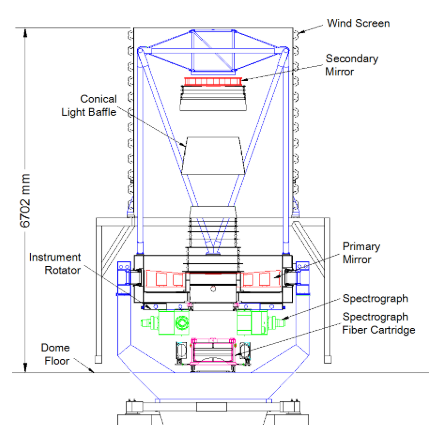
\includegraphics[scale=0.5]{SchemaTelescope}
  \caption{Schéma du télescope SDSS. Le miroir principal est représenté en bas en rouge. Le miroir secondaire est visible au sommet du télescope en rouge. Les spectrographes sont représentés en vert sous le télescope. Une cartouche, pas encore disposée au plan focal du télescope, est représentée sous les spectrographes. Crédits :~\textcite{Smee2012}.}
  \label{fig:SchemaTelescope}
\end{figure}
Le télescope se compose d'un miroir primaire de $\SI{2,5}{\meter}$ de diamètre et d'ouverture f/\num{2,25}, et d'un miroir secondaire de $\SI{1,08}{\meter}$ de diamètre situé à $\SI{3,6}{\meter}$ du miroir primaire. Avec un plan focal situé à $\SI{0,76}{\meter}$ derrière le miroir primaire, l'ouverture finale du télescope est f/5. Le champ de vue qui en résulte est de $\SI{3}{\deg}$ de diamètre sur le ciel ($\SI{7}{\square\deg}$), correspondant à un diamètre de $\SI{0,65}{\meter}$ dans le plan focal. \\
Le télescope inclut aussi 2 correcteurs optiques. Le premier est un correcteur d'astigmatisme de type Gascoigne. Le second est un jeu de correcteurs hautement asphériques et interchangeables situés près du plan focal. L'un, épais, est utilisé pour la photométrie ; l'autre, beaucoup plus fin, est utilisé lors des phases de spectrométrie.


\subsubsection{La caméra}
L'instrument nécessite une caméra \autocite{Gunn1998} capable de couvrir l'entièreté du plan focal du télescope. Le très grand champ de vue du télescope a imposé l'utilisation des CCD les plus grands disponibles à l'époque : les Tektronix Tk2048E. Ces CCD sont des grilles de \num{2048x2048} pixels de $\SI{24}{\micro\meter}$. Etant donné la longueur focale du télescope, ces $\SI{24}{\micro\meter}$ représentent $\SI{0,4}{\arcsecond}$ sur le ciel. Ainsi, la PSF\footnote{La PSF (\emph{Point Spread Function}) désigne la réponse d'un système optique à une source ponctuelle.} d'une largeur à mi-hauteur d'environ $\SI{1}{\arcsecond}$ est bien échantillonnée. \\
La caméra est constituée de 2 modules, le premier comportant 5 (filtres\footnote{Il s'agit des 5 filtres u, g, r, i et z. Voir figure~\ref{fig:Filtres}}) x 6 (colonnes) CCD est destiné à la photométrie. En plus de ces 30 CCD, 22 CCD \num{400x2048} et de même taille de pixel sont ajoutés au dessus et en dessous du module dédié à la photométrie. Ces CCD permettent de relier les étoiles standards brillantes aux objets observés lors de la phase photométrique. Ils constituent le module d'astrométrie. Deux CCD supplémentaires sont ajoutés comme dispositif de contrôle pour la mise au point. La figure~\ref{fig:CcdSchema} résume leur disposition.
\begin{figure}
  \centering
  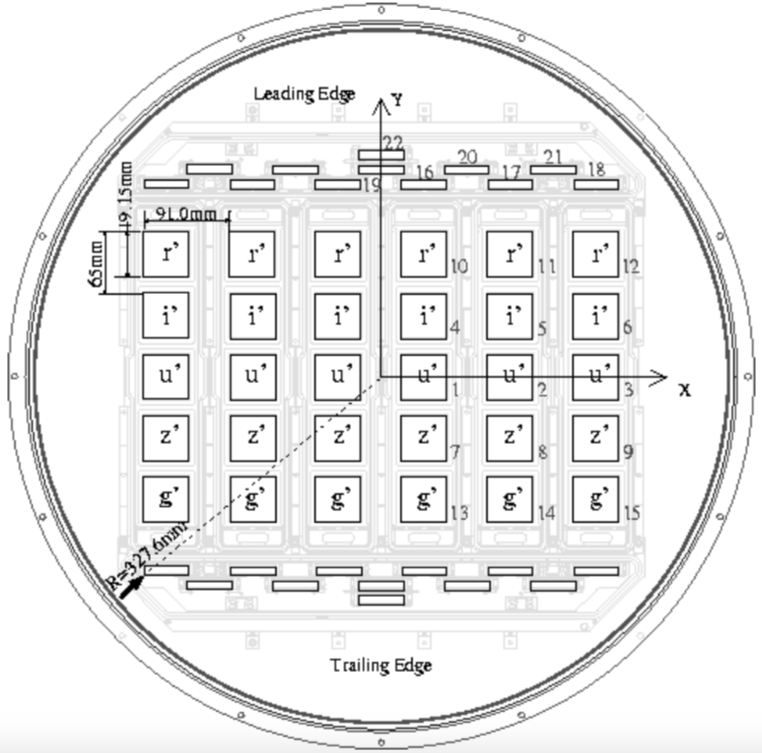
\includegraphics[scale=0.3]{CcdSchema}
  \caption{Schéma de la disposition des CCD dans le plan focal du télescope SDSS. Les capteurs 1 à 15 sont les CCD dédiés à la photométrie. Le module d'astrométrie se compose des CCD 16 à 21. Enfin le CCD 22 sert au contrôle de la mise au point.}
  \label{fig:CcdSchema}
\end{figure}

\begin{figure}
  \centering
  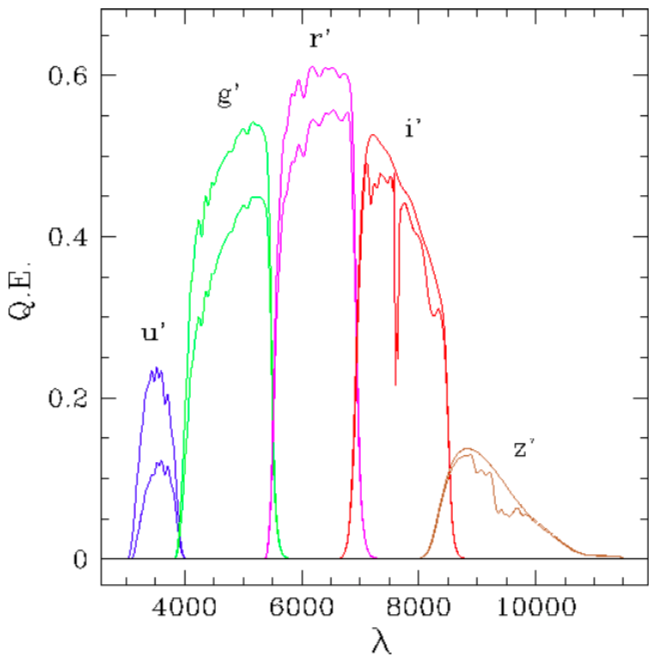
\includegraphics[scale=0.4]{Filtres}
  \caption{Efficacité de chacun des 5 filtres utilisés lors de la phase photométrique de SDSS. Les courbes incluent l'efficacité quantique des CCD, ainsi que l'efficacité du système optique. Les courbes en dessous incluent en plus la transmission de l'atmosphère.}
  \label{fig:Filtres}
\end{figure}

Lors de la phase d'observation photométrique, la caméra est utilisée en mode \emph{time delay integration} (TDI). Ce mode d'observation consiste à laisser le ciel défiler devant la caméra. La lumière de chaque objet est ainsi accumulée durant tout le transit de l'objet. Cette technique permet de gagner en efficacité d'observation, en réduisant le temps de lecture (qu'il y aurait en mode exposition classique) et le temps de pointage du télescope.


\subsubsection{Le spectrographe}

Une fois la phase de photométrie effectuée et les cibles sélectionnées, la phase de spectroscopie commence.
Les plaques d'observations sont d'abord percées aux positions des cibles dans le plan focal.
Ces plaques sont ensuite disposées au plan focal du télescope (à la place de la camera). Les fibres, insérées dans ces plaques et placées à la position de chaque cible, sont ensuite envoyées vers les spectrographes \autocite{Smee2012} afin de mesurer le spectre de ces cibles.

Les spectrographes utilisés dans eBOSS sont les mêmes que ceux utilisés dans BOSS. Ces spectrographes, initialement présents dans SDSS, ont été améliorés afin d'atteindre les objectifs de BOSS. Comparé à SDSS, BOSS a augmenté le nombre de spectres mesurés de \SI{35}{\percent}, ses objets étant à plus grand redshift, donc de plus faible luminosité. Ainsi le nombre de fibres des spectrographes de BOSS passe de \num{640} à \num{1000}. Les objets observés étant plus lointains et donc ayant une taille sur le ciel plus petite, le diamètre de ces fibres est réduit d'un tiers, passant à $\SI{120}{\micro\meter}$, afin d'augmenter le rapport signal sur bruit des spectres. BOSS inclut aussi un nouveau traceur : la forêt \lya{}. Afin de mesurer l'absorption dans la forêt \lya{} des quasars à un redshift $z=\num{2,2}$, la longueur d'onde d'observation minimale a été diminuée de \num{3900} à $\SI{3560}{\angstrom}$. De la même manière, la longueur d'onde d'observation maximale à été augmenté de \num{9100} à $\SI{10400}{\angstrom}$ pour améliorer la détermination des redshifts de l'échantillon de galaxies.

\paragraph{} Pour limiter les risques de dommage aux fibres lors du montage et du démontage des différentes plaques, chaque plaque est montée sur un support rigide. Ce support rigide est appelé cartouche, il comporte la plaque d'observation en aluminium, les \num{1000} fibres insérées dans cette plaque, et deux \emph{slitheads} qui sont ensuite insérés dans chacun des spectrographes. La figure~\ref{fig:CartoucheImage} donne un apperçu de ces cartouches.\\
\begin{figure}
  \centering
  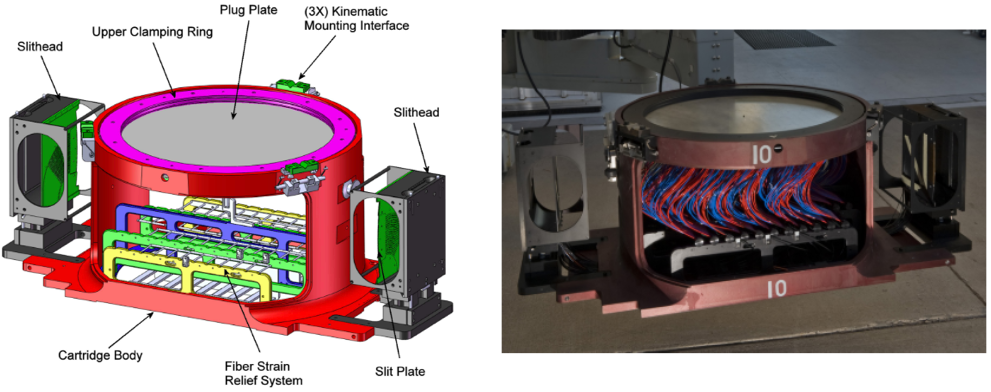
\includegraphics[scale=0.35]{CartoucheImage}
  \caption{Le schéma de gauche présente les différents éléments d'une cartouche. On peut y reconnaître la plaque en aluminium sur le dessus en gris. Sur la droite, une photo d'une cartouche sur laquelle les fibres optiques ont été insérées dans la plaque d'aluminium. L'extrémité des fibres est reliée aux slitheads, visibles à droite et à gauche, qui seront insérés dans les 2 spectrographes. Crédits : \textcite{Smee2012}.}
  \label{fig:CartoucheImage}
\end{figure}
L'instrument dispose de deux spectrographes. Ils sont schématisés sur la figure~\ref{fig:SchemaSpectro}.
% Chacun des spectrographes reçoit via les slitheads \num{500} fibres optiques.
Les \num{1000} fibres d'une plaque sont séparées en deux. Chaque lot de \num{500} fibres constitue une \emph{demi-plaque}. Chaque spectrographe reçoit donc les fibres optiques d'une demi-plaque, via les slitheads.
La lumière issue de ces fibres est collimatée grâce à un miroir sphérique. Le faisceau parallèle ainsi créé passe à travers un miroir semi-réfléchissant, permettant de séparer les longueurs d'onde plus petites que $\SI{6050}{\angstrom}$ des longueurs d'onde plus grandes. Enfin, chaque demi-faisceau passe au travers d'un grisme\footnote{Association d'un prisme et d'un réseau de diffraction. Le grisme permet de décomposer la lumière tout en gardant le faisceau parallèle.}, et arrive sur la caméra bleue pour les longueurs d'onde plus petites que $\SI{6050}{\angstrom}$, ou sur la caméra rouge pour les longueurs d'onde plus grandes. 
Après avoir traversé toutes les pièces d'optique, la lumière arrive sur des CCD de \num{4000x4000} pixels, avec une taille de pixel de $\SI{15}{\micro\meter}$. Ainsi une des dimensions du CCD correspond à la longueur d'onde observée, selon l'axe de dispersion, l'autre dimension parcours les différentes fibres. Selon cette dimension, chaque spectre possède un profil de 3 pixels de large et  est séparé de son voisin par 6 pixels afin d'éviter la contamination d'un spectre à un autre.
\begin{figure}
  \centering
  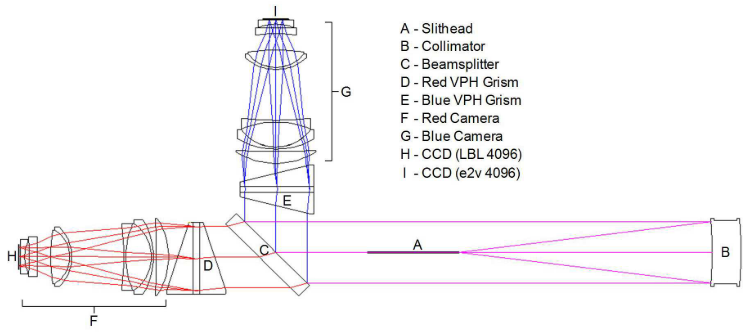
\includegraphics[scale=0.5]{SchemaSpectro}
  \caption{Schéma des spectrographes de BOSS. La lumière arrive via les fibres optiques (A). Elle est ensuite collimatée (B) en un faisceau parallèle, puis séparée par le mirroir semi-réfléchissant (C). Les longueurs d'ondes $\lambda < \num{6050}$ sont réfléchies vers la caméra bleu (G), les autres entrent dans le bras rouge (F) du spectrographe. Chaque bras comporte un grisme (D et E), une série de lentille puis le CCD (H et I). Crédits : \textcite{Smee2012}.}
  \label{fig:SchemaSpectro}
\end{figure}

\subsubsection{Les performances}
Les améliorations apportées à l'instrument pour BOSS ont permis d'augmenter le nombre maximal de spectres observables par nuit, ainsi que la magnitude limite atteignable. Cette dernière est directement liée à l'efficacité optique du système. L'efficacité optique est définie comme le ratio du flux mesuré d'une source ponctuelle sur le flux de cette même source situé en dehors de l'atmosphère. La figure~\ref{fig:SpectroThroughput} présente les estimations des différentes composantes participant à l'efficacité optique globale de l'instrument. %, ainsi que la comparaison entre l'efficacité optique mesuré pour SDSS et pour BOSS, en fonction de la longueur d'onde. Grâce aux améliorations apportées pour BOSS, l'efficacité optique a été multipliée par environ un facteur 2.
\begin{figure}
  \centering
  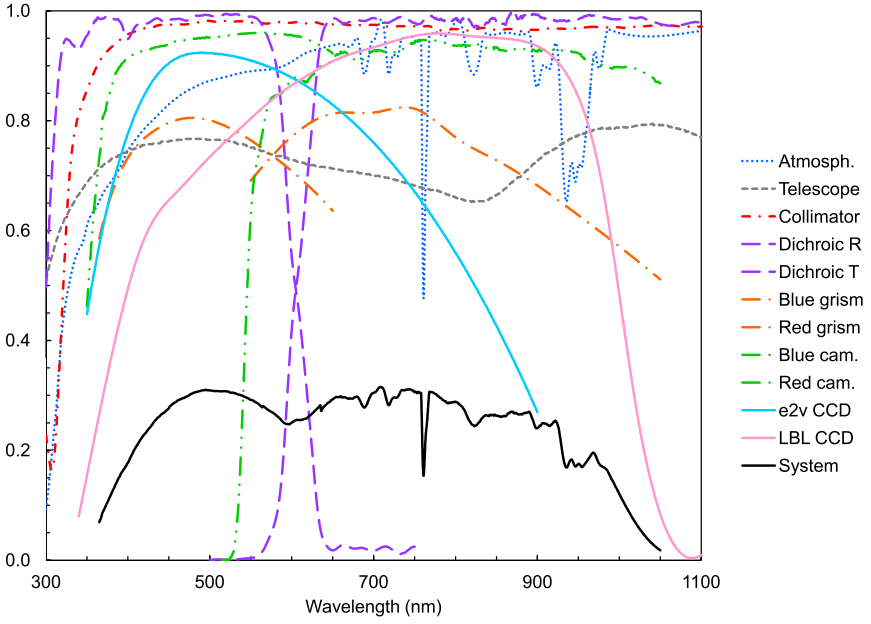
\includegraphics[scale=0.35]{SpectroThroughput}
  % \caption{Efficacité optique en fonction de la longueur d'onde. Le panneau de gauche présente les prévisions de l'efficacité optique de l'instrument avec toutes ses composantes. Le panneau de droite présente l'efficacité optique du spectrographe 1 (en haut) et du spectrographe 2 (en bas) de SDSS (noir) et de BOSS (rouge). Crédits :~\cite{Smee2012}. \#prov Est-ce que c'est bien visible la fig de droite ?}
  \caption{Efficacité optique en fonction de la longueur d'onde. Le graphique présente les prévisions de l'efficacité optique de l'instrument avec toutes ses composantes. Crédits : \textcite{Smee2012}.}
  \label{fig:SpectroThroughput}
\end{figure}

Le pouvoir de résolution traduit la capacité de l'instrument à identifier et mesurer des raies spectrales. Pour mesurer ce pouvoir de résolution, le spectre de lampes à arc dédiées à la calibration est mesuré, puis chaque raie d'émission est ajustée par une gaussienne de largeur $\sigma_\lambda$. Ce $\sigma_\lambda$ est ensuite ajusté par un polynome en fonction de $\lambda$, ce qui donne une estimation de la largeur d'une raie spectrale en fonction de la longueur d'onde observée.
Enfin, le pouvoir de résolution est défini comme $R = \frac{\lambda}{FWHM}$, où la largeur à mi-hauteur FWHM (pour \emph{Full Width at Half Maximum}) vaut $\num{2.36}\sigma_{\lambda}$ et donne la résolution de l'instrument.
% La résolution est donnée par le dénominateur : la largeur à mi-hauteur de la gaussienne.
Le pouvoir de résolution a été mesuré sur \num{100} plaques SDSS et \num{100} plaques BOSS. La comparaison est présentée sur la figure~\ref{fig:SpectroResoPower}. Le pouvoir de résolution est légèrement moins grand pour BOSS que pour SDSS, mais reste au dessus des prérequis.
\begin{figure}
  \centering
  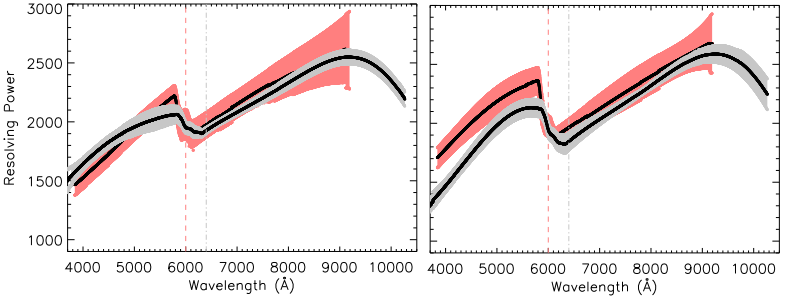
\includegraphics[scale=0.5]{SpectroResoPower}
  \caption{Pouvoir de résolution en fonction de la longueur d'onde pour les spectrographes de SDSS (rouge) et BOSS (gris). La courbe de gauche correspond à la mesure sur le spectrographe 1, et celle de droite sur le spectrographe 2. Les régions colorées représentent les régions contenant \SI{68}{\percent} des mesures. Crédits : \textcite{Smee2012}.}
  \label{fig:SpectroResoPower}
\end{figure}


\newpage
\subsection{Résultats}
Le relevé eBOSS fournit les mesures de l'échelle BAO et du taux de croissance $f \sigma_8$ les plus précises à ce jour. Ces mesures, grâce à la diversité de traceurs utilisés, sont réparties dans une large gamme en redshift, allant de $z \sim 0.15$ avec les galaxies locales à $z \sim 2.4$ avec le \lya{}.
La figure~\ref{fig:exp_hist} présente l'ensemble de ces mesures.
Parmi les nombreux résultats produits par eBOSS, nous pouvons citer la mesure de l'échelle BAO qui favorise une densité d'énergie noire non nulle à plus de 8 sigmas. % de la densité d'énergie noire qui est non nulle à plus de 8 sigmas.
La figure~\ref{fig:olambda_om} montre les contraintes sur les paramètres $\Omega_{\Lambda}$ et $\Omega_{m}$ apportées uniquement par la mesure de l'échelle BAO.
En ajoutant les mesures de la BBN (\emph{Big Band Nucleosynthesis}), la mesure de l'échelle BAO faite par eBOSS produit une mesure de $H_0$ en accord avec les mesures de Planck, et en tension avec les mesures directes.
La figure~\ref{fig:h0_om} montre les contraintes sur les paramètres $H_0$ et $\Omega_{m}$ apportées par la mesure de l'échelle BAO. La combinaison des mesures à $z > 1$ et $z < 1$ permet de mesurer précisément à la fois $H_0$ et $\Omega_{m}$. La zone horizontale grise montre la mesure directe de $H_0$ faite par~\textcite{Riess2019}.
Enfin, eBOSS permet de réduire la limite supérieure de la somme des masses des neutrinos à $\num{0.115}\; \mathrm{eV}$.
Tous les résultats et contraintes cosmologiques produits par eBOSS sont présentés et discutés dans~\textcite{EBOSSCollaboration2020}.


\begin{figure}
  \centering
  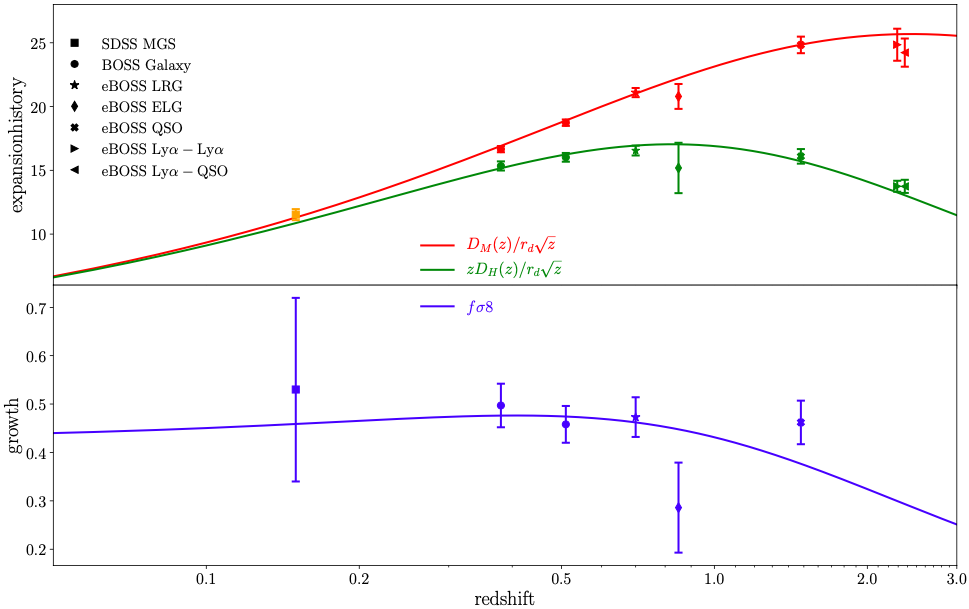
\includegraphics[scale=0.42]{exp_history}
  \caption{L'ensemble des mesures de l'échelle BAO (graphique du haut) et du taux de croissance $f \sigma_8$ (graphique du bas) produites par tous les relevés SDSS. Les lignes continues indiquent les prédictions produites par Planck en supposant un modèle \lcdm{} plat.}
  \label{fig:exp_hist}
\end{figure}

\begin{figure}
  \centering
  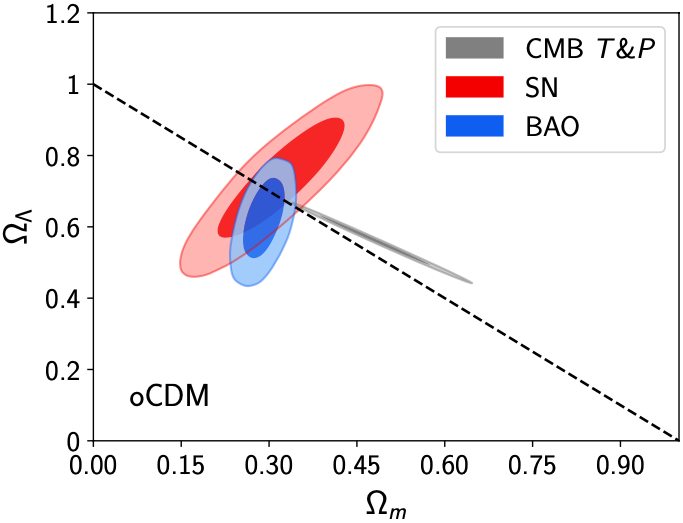
\includegraphics[scale=0.45]{olambda_om}
  \caption{Contraintes cosmologiques sur les paramètres $\Omega_{\Lambda}$ et $\Omega_{m}$, avec l'hypothèse d'un modèle \lcdm{} de courbure libre. Les contours rouges indiquent les contraintes à 1 et 2 sigmas produites à partir des données du relevé de supernovae Pantheon \autocite{Scolnic2017}, les gris indiques les contraintes produites par Planck (température et polarisation), et les bleus donnent les contraintes produites par la mesure de l'échelle BAO avec l'ensemble des relevés SDSS.}
  \label{fig:olambda_om}
\end{figure}

\begin{figure}
  \centering
  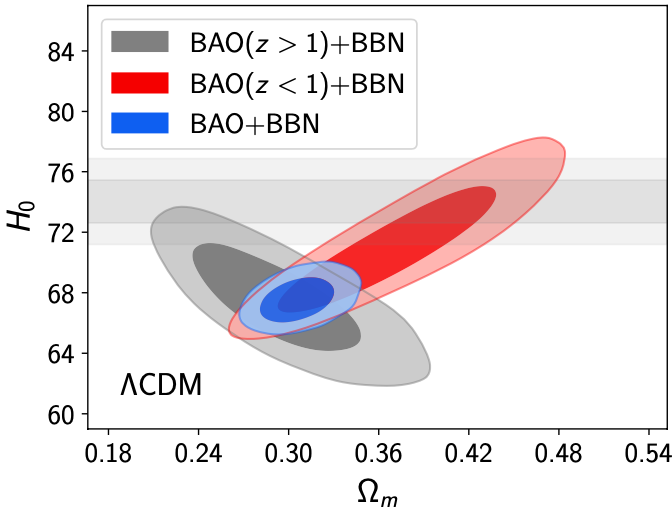
\includegraphics[scale=0.45]{hzero_om}
  \caption{Contraintes cosmologiques sur les paramètres $H_0$ et $\Omega_{m}$ produites par la mesure de l'échelle BAO avec l'ensemble des relevés SDSS, en supposant un modèle \lcdm{} plat. Les contours rouges et gris indiquent les contraintes à 1 et 2 sigmas produites par les mesures à $z > 1$ et $z < 1$ respectivement. Les contours bleus indiquent la combinaison de tous les mesures. Enfin, la zone horizontale grise montre la mesure de $H_0$ faite par \textcite{Riess2019}.}
  \label{fig:h0_om}
\end{figure}


\section{DESI}

Le \emph{Dark Energy Spectroscopic Instrument} (DESI, \textcite{DESICollaboration2016}) est un projet américain de mesure d'énergie noire de génération 4.
Il a vu sa première lumière en octobre 2019. % et devrait commencer la prise de données en juillet 2020. (\#prov Commissionning octobre 2019 - fev 2020 puis 3 mois de SV pour tester la TS, qualité des spectres pour la détermination du redshift (temps d'exposition), puis dernier mois de SV o\`u on fait \SI{1}{\percent} du survey avec la config choisie (TS entre autre). A la fin de ce mois là, soit on garde et on continue le survey, soit on retouche la TS par exemple, et on part pour le survey (dans ce cas le \SI{1}{\percent} est perdu).)
Le début de la prise de données devait avoir lieu en juillet 2020. Cependant, à cause de la pandémie de 2020, les phases de \emph{commissioning} et \emph{survey validation} durant laquelle l'instrument et  la qualité des données sont testés ont été intérompues. Actuellement, le début de la prise de données est estimé à janvier 2021.


Comme eBOSS, DESI étudie les BAO et la croissance des structures à l'aide d'un très grand relevé de galaxies et de quasars. A l'issue des 5 ans d'observation prévus, DESI aura mesuré plus de 30 millions de spectres, distribués sur un relevé de plus de $\SI{14000}{\square\deg}$.
Pour atteindre ses objectifs, DESI utilise le télescope Mayall, mesurant $\SI{4}{\meter}$ de diamètre et situé au Kitt Peak en Arizona. Le champ de vue du télescope est le même que celui de SDSS : $\SI{3}{\deg}$ de diamètre sur le ciel. L'instrument inclut un système de fibres optiques, au nombre de \num{5000}, mais celles-ci sont placées au plan focal à l'aide de robots qui ajustent la position de chaque fibre avant chaque exposition. Dix spectrographes reçoivent ces fibres, chacun comportant 3 caméras et couvrant les longueurs d'onde de \num{3600} à $\SI{9800}{\angstrom}$.
% L'instrument inclut \num{5000} fibres, dont le placement au plan focal est robotisé. Les fibres sont envoyés vers 10 spectrographes, chacun comportant 3 caméras et couvrant les longueurs d'onde de \num{3600} à $\SI{9800}{\angstrom}$. \\
‌‌DESI observe les 4 mêmes traceurs qu'eBOSS : les LRG jusqu'à $z=\num{1,0}$, les ELG jusqu'à $z=\num{1,7}$, ainsi que les quasars en tant que traceurs directs de la matière et les quasars \lya{} sur la gamme $\num{2,1} < z < \num{3,5}$. La densité visée de quasars \lya{} est de \num{50} par $\si{\square\deg}$.
En plus de ces traceurs, DESI observera des galaxies brillantes (BG : \emph{Bright Galaxies}) pendant le grey time\footnote{Le grey time, par opposition au dark time, correspond au moment où le ciel n'est pas totalement sombre, lorsqu'il est éclairé par la lune par exemple.}. Le relevé de ces galaxies contiendra 10 millions d'objets, avec un redshift moyen $z=\num{0,2}$.

A la fin des 5 ans d'observations, DESI fournira plus de 30 points de mesure des distances cosmologiques, chacun avec une précision meilleure que le pourcent, et couvrant la gamme $\num{0}< z < \num{3.5}$. La figure~\ref{fig:DesiVsEboss} illustre la différence entre BOSS et DESI pour la mesure du taux d'expansion $H(z)$.
De plus, DESI donnera une mesure de la somme des masses des neutrinos, avec une incentitude de $\num{0,020}\,\mathrm{eV}$. Cette précision est suffisante pour exclure la hiérarchie de masse inversée à $3\,\sigma$.


\begin{figure}
  \centering
  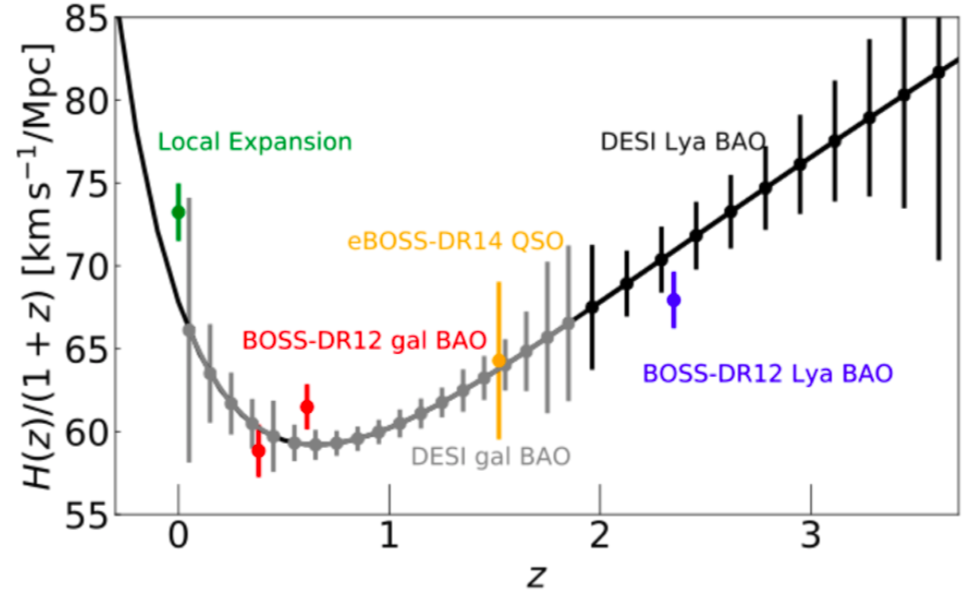
\includegraphics[scale=0.3]{DesiVsEboss}
  \caption{Mesure de la distance de Hubble en fonction du redshift. Les points vert (mesure local \`a l'aide des SN1a), rouge, jaune et bleu donnent les mesures existantes. Les points gris donnent la prédiction pour les galaxies et quasars de DESI, les points noirs donnent la prédiction pour le \lya{} de DESI.}
  \label{fig:DesiVsEboss}
\end{figure}

% \bibliography{../source/library}
% \printbibliography
% \end{document}
